\documentclass[../full_thesis/full_thesis.tex]{subfiles}

% Default image directory
\newcommand{\thisdir}{../inertial_frame}
\graphicspath{{\thisdir/img/}}


\begin{document}

In Sec.~\ref{sec: rotating frame} we developed our intuition for the precession
of neutron stars by working in the rotating body frame of the star.  However,
pulsar astronomers report on physical observations of the star made in the
inertial frame, in particular those quantities calculable from the radio
pulsations. Therefore, in this section we will develop our model by making
predictions for how precession manifests in the observable features of a
pulsar. This will require us to understand and make a model for how the
observations are made by pulsar astronomers.  We will use both exact numerical
solutions and analytic approximations: the numerical solutions allow us to
verify the analytic approximations and furthermore will allow us to introduce
new features into the model with no analytic analogue.

\section{Rotating into the inertial frame}

The Euler rigid body equation of Eqn.~\eqref{eqn: eom} are defined in the
rotating body frame of the star. To discuss results in the inertial frame of
an observer, we need to transform the solutions of Euler's rigid body equations
into the inertial frame.  An efficient way to do this
is to determine the Euler angles which transform the rotating body frame axis,
denoted by $(x',y', z')$, to the inertial frame axis for which we will use $(x,
y, z)$. In particular, we will use the Euler angle parameterisation as described by
\citet{Landau1969}; a schematic of how these angles are constructed is given in
Fig.~\ref{fig: Euler}.
\begin{figure}[ht]
\centering
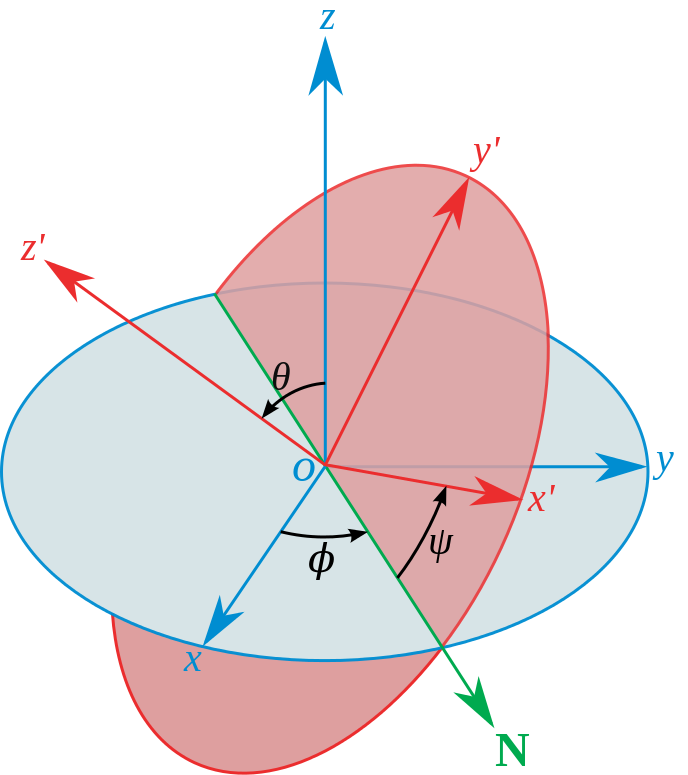
\includegraphics[scale=0.25]{Eulerangles-alternative_filled.png}
% http://commons.wikimedia.org/wiki/File:Eulerangles-alternative.svg
\caption{Schematic of the Euler rotation angles between the rotating body
frame $(x', y', 'z')$ and the inertial frame $(x, y, z)$.}
\label{fig: Euler}
\end{figure}

In Eqn.~\eqref{eqn: rotation matrix} we define the Euler angle rotation matrix;
following the \citet{Landau1969} convention
\begin{equation}
R(\theta, \phi, \psi) = \left[
\begin{array}{ccc}
\cos\psi \cos\phi - \cos\theta \sin\phi \sin \psi &
\cos\psi \sin \phi + \cos\theta \cos \psi \sin \psi &
\sin \psi \sin\theta \\
-\sin\psi \cos\phi - \cos\theta\sin\phi\cos\psi &
-\sin\psi\sin\phi + \cos\theta\cos\phi\cos\psi &
\cos\psi \sin\theta \\
\sin\theta\sin\phi &
-\sin\theta \cos\phi &
\cos\theta
\end{array}
\right].
\label{eqn: rotation matrix}
\end{equation}

The Euler angles are defined via a set of three ODEs which are coupled both to
the other Euler angles and the components of the spin-vector. To have solutions
both for the motion of the spin-vector in the rotating frame and the Euler
angles we need to solve all six ODEs together. To be specific, the six ODEs are
given in equations~\eqref{eqn: ODEs}: the in left-hand triplet is the
components of the Euler rigid body equations first given in Eqn.~\eqref{eqn:
EOM}; in the right-hand triplet we give the rearranged set of Euler angles ODEs
from \citet{Landau1969}.
\begin{align}
\begin{split}
\dot{\omega_{x}} & = \frac{1}{I_{xx}}\left[T_{x} +
                      \left(I_{yy} - I_{zz}\right) \omega_{y} \omega_{z}\right],
\\
\dot{\omega_{y}} & = \frac{1}{I_{yy}}\left[T_{y} +
                      \left(I_{zz} - I_{xx}\right) \omega_{x} \omega_{z}\right],
\\
\dot{\omega_{z}} & =\frac{1}{I_{zz}}\left[T_{z} +
                      \left(I_{xx} - I_{yy}\right) \omega_{x} \omega_{y}\right],
\end{split}
\begin{split}
\dot{\phi} & = \frac{\omega_{x} \sin \psi + \omega_{y} \cos \psi}{\sin \theta},\\
\dot{\theta} & = \omega_{x} \cos \psi - \omega_{y} \sin \psi,\\
\dot{\psi} & = \omega_{z} - \dot{\phi} \cos \theta.
\end{split}
\label{eqn: ODEs}
\end{align}
This set of six coupled ODEs can be solved numerically using a time stepper, we
will use the \texttt{rkf45} stepper provided by GSL \citep{gough2009gnu}.
Solutions give the components of the spin-vector in the rotation frame and the
evolution of the Euler angles which can be used to transform body-frame
quantities into the inertial frame. Unlike the results of Sec.~\ref{sec:
rotating frame}, numerical solutions to these ODEs require the fast spin frequency
to be resolved and hence require greater computing time.

The rotation period of the star is several orders of magnitude smaller than the
precession period, as a result the Euler angles evolve on a much shorter time
scale than the body frame spin components. This is numerically expensive. To
allow efficient investigations we will therefore consider unrealistic values to
understand the different types of motion before using realistic values only in
cases of interest.

\section{Initial conditions}

Solving the rigid body equations, as in Sec.~\ref{sec:
rotating frame}, we impose the following initial conditions on the
spin vector
\begin{align}\label{eqn: spin init}
\omega_{x} & = \omega_{0}\sin(a_{0}), &
\omega_{y} & = 0, &
\omega_{z} & = \omega_{0}\cos(a_{0}),
\end{align}
such that $\spin(t=0)$ lies in the $x' - z'$ plane at an angle $a_{0}$ to the
$z'$ axis.

For the Euler angle equations, the right-hand triplet in Eqn.~\eqref{eqn:
ODEs}, the initial conditions need to be chosen carefully so that the result
can be meaningfully interpreted. In particular we need to be sure we understand
how the inertial frame is orientated. To do this, we note that the angular
momentum in the two frames are related by
\begin{equation}
\Jr = R(\theta, \phi, \psi) \Ji .
\label{eqn: transform}
\end{equation}
where $R(\theta, \phi, \psi)$ is defined in Eqn.~\eqref{eqn: rotation matrix}.

In the body frame, the moment of inertia is constant, ignoring small variations
due to the fact that the torque is not parallel to the angular momentum.
We have already set the initial condition on $\spin$  in Eqn.~\eqref{eqn:
spin init}, therefore the initial angular momentum in the rotating frame is given by
\begin{equation}
  \Jr(t=0) = I \spin_0.
\end{equation}
If we set an initial condition on the angular momentum in the inertial frame
$\Ji$ then Eqn.~\eqref{eqn: rotation matrix} uniquely defines the initial
Euler angles. We choose to set the initial angular momentum in the inertial
frame to lie along the inertial $z$ axis such that
\begin{equation}
  \Ji(t=0) = |\Ji| \mathbf{z}.
\end{equation}
The magnitude of the angular momentum is
\begin{equation}
|\J| = |I \spin_{0}|=\omega_{0}\sqrt{(I_{xx}\sin a_{0})^{2} + (I_{zz}\cos a_{0})^{2}},
\end{equation}
then from Eqn.~\eqref{eqn: transform} we have
\begin{equation}
\left[ \begin{array}{c}
I_{xx}\sin a_{0} \\
0 \\
I_{zz} \cos a_{0}
\end{array}\right] =
\sqrt{(I_{xx}\sin a_{0})^{2} + (I_{zz}\cos a_{0})^{2}}
\left[ \begin{array}{c}
\sin \psi_{0} \sin \theta_{0} \\
\cos \psi_{0} \sin \theta_{0} \\
\cos \theta_{0}
\end{array}\right].
\label{eqn: 010203}
\end{equation}•
We have three equations for two unknowns. Our choice to set $\J$ along
the $z$ axis leaves the initial value of $\phi$ a free variable,
we set $\phi_{0} = 0$.
Rearranging the third component of Eqn.~\eqref{eqn: 010203} yields
\begin{equation}
\theta_{0} = \arccos\left(\frac{I_{zz}\cos a_{0}}{ \sqrt{(I_{xx}\sin
        a_{0})^{2} + (I_{zz}\cos a_{0})^{2}}} \right).
\label{eqn: theta init}
\end{equation}
In the limit $\epsilon_{I} \ll 1$ we have that $\theta_{0} \approx a_{0}$.
For $\psi_0$, we rearrange the first component of Eqn.~\eqref{eqn: 010203} to
give
\begin{equation}
\sin\psi_{0} =\frac{1}{ \sin\theta_{0}}
\frac{ I_{xx}\sin a_{0}}{\sqrt{(I_{xx}\sin a_{0})^{2} + (I_{zz}\cos a_{0})^{2}}}.
\label{eqn: 8283}
\end{equation}
To simplify the first factor we use the identity $\sin(\arccos(x)) = \sqrt{1 - x^{2}}$
along with Eqn.~\eqref{eqn:  theta init} giving
\begin{equation}
\sin\theta_{0} = \left(\frac{(I_{xx}\sin a_{0})^{2}}
                  {(I_{xx}\sin a_{0})^{2} + (I_{zz}\cos a_{0})^{2}} \right)^{1/2}.
\end{equation}
Inserting this into Eqn.~\eqref{eqn: 8283} and rearranging we find that
\begin{align}
\sin \psi_0 & = \frac{I_{xx} \sin a_{0}}{\left(I_{xx}^{2} \sin^{2} a_{0}\right)^{1/2}} \\
 & = \frac{\sin a_{0} }{|\sin a_{0}|} \\
& = \mathrm{sign}(a_{0}),
\end{align}
where by $\mathrm{sign}(x)$ we mean the sign of $x$. Finally, the initial
condition is given by
\begin{align}
\psi_{0} & =\mathrm{sign}(a_{0}) \frac{\pi}{2}.
\label{eqn: psi  init}
\end{align}
We can check the sanity of this result by inserting it into the second component of
Eqn.~\eqref{eqn: 010203} and finding that it balances the right hand side.

In this section we have defined the appropriate initial conditions for the system.
While the initial conditions on the spin-vector are arbitrary, if the initial
Euler angle are not carefully defined then we do not have a meaningful interpretation
for how the inertial frame is orientated.

\section{Dynamics of the magnetic dipole}

Numerical solutions to Eqn.~\eqref{eqn: ODEs} allow us to calculate the motion
of any quantity in the inertial frame from which the neutron star is observed.
This can be used for example to calculate the motion of the spin-vector in the
rotating frame under any torque. However, pulsar astronomers observe the pulsar
through the pulsations of EM emission. If this emission is colinear with the
dipole, then it points along the unit vector of the magnetic dipole $\m$. Therefore
we are particular interested in the motion of $\m$ in inertial frame. Before

In the body frame we set $\m$ to lie at an angle $\chi$ to the $z'$ axis with
unit vector $[\sin(\chi), 0, \cos(\chi)]$. Using the Euler angles rotation
matrix, \eqref{eqn: rotation matrix}, to transform to the inertial frame, the
components are given by
\begin{equation}
\m =
\left[\begin{array}{c}
\cos\phi\cos\psi\sin\chi - \sin\phi \cos \theta \sin \psi \sin \chi
+ \sin \phi \sin \theta \cos \chi \\
\sin\phi\cos\psi\sin\chi + \cos\phi \cos \theta \sin \psi \sin \chi
- \cos \phi \sin \theta \cos \chi \\
\sin\theta \cos\psi \sin\chi + \cos\theta \cos \chi
\end{array}\right].
\label{eqn: m inertial}
\end{equation}•
Following the work of \citet{Jones2001} two angles $\Phi$ and $\Theta$ are
defined to describe the polar and azimuth of $\m$ in the inertial frame.
The azimuthal angle is given by
\begin{equation}
    \Phi = \arctan\left(\frac{\m_{y}}{\m_{x}}\right) =
\phi - \frac{\pi}{2} + \arctan\left(\frac{1}{\cos\theta}
                       \left(\frac{\cos\psi \tan \chi}{\tan\theta -
                       \sin \psi \tan\chi }\right)\right),
\label{eqn: Phi}
\end{equation}
while the polar angle is
\begin{equation}
\Theta = \arccos(\m_{z}) = \arccos(\sin \theta \sin \psi \sin \chi + \cos \theta \cos \chi ).
\label{eqn: Theta 2}
\end{equation}

Given a numerical solution of equations~\eqref{eqn: ODEs} we can use these two
equations to describe the evolution of the magnetic dipole orientation in the
inertial frame. Before doing so, we will consider what can be learnt analytically
in the torque free case.

\section{Dynamics of the magnetic dipole: torque free precession}
\label{sec: understanding the motion of m}

The solutions to equations~\eqref{eqn: ODEs} were studied by \citet{Jones2001}
where it was found that the Euler angles had simple analytic solutions given by
\begin{align}
\begin{split}
    \theta(t) & = \theta_{0} \approx a_{0} \\
    \phi(t) & = \dot{\phi}t + \phi_{0} = \omega_{z} t \\
    \psi(t) & = \dot{\psi}t + \psi_{0}= -\epsilon_{I}\omega_{z}t+\frac{\pi}{2}
\end{split}
\label{eqn: euler angles torque free evolution}
\end{align}
while we gave the solutions to the rigid body equations in Eqn.~\eqref{eqn:
free precession}.

From Eqn.~\eqref{eqn: rotation matrix} we can use these solutions to calculate
the motion of vectors fixed in the rotation body frame, such as the magnetic
dipole, in the inertial frame. The resulting expression can display a rich
variety of behaviours, but these can be understood by first decomposing the
spin-vector into rotations about the angular momentum and rotation about the
deformation axis:
\begin{equation}
  \spin = \dot{\phi}\n_{J} + \dot{\psi}\n_{d}.
\label{eqn: decomp}
\end{equation}
Any fixed vector in the body frame can be understood, in the inertial frame, as
undergoing two motions: keeping $\phi$ fixed and increasing $\psi$ rotates the
vector in a cone about the $\n_{d}$ axis; holding instead $\psi$ fixed and
increasing $\phi$ sweeps the vector about a cone centred around the $\n_{J}$
axis. Calling these cones the precession and spin cones respectively the
resulting motion can be understood as the superposition of the two.

\citet{Jones2001} found that the types of solutions these cones produced
depended on the ordering of $\theta$ and $\chi$. To understand why this is, in
Fig.~\ref{fig: cones} we provide three illustrations of the two cones projected
into the reference plane for the three possible orderings of $\theta$ and $\chi$.
\begin{figure}[ht]
\centering
	\subfloat[$\chi < \theta$]{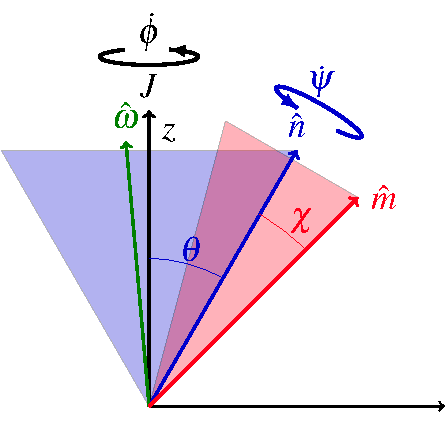
\includegraphics[width=0.33\textwidth]
    {chi_less_theta.pdf}}
	\subfloat[$\chi = \theta$]{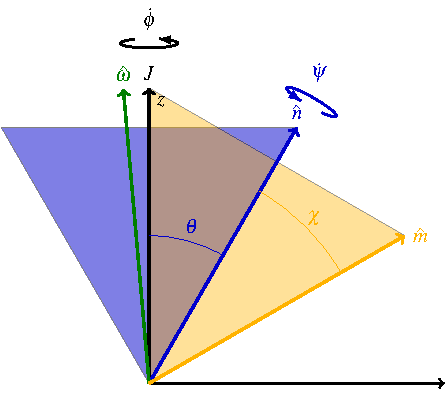
\includegraphics[width=0.33\textwidth]
    {chi_equal_theta.pdf}}
	\subfloat[$\chi > \theta$]{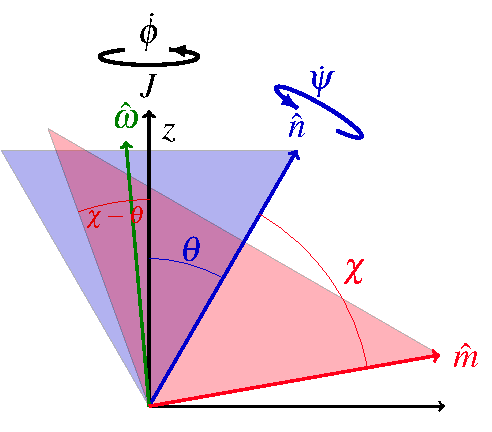
\includegraphics[width=0.33\textwidth]
    {chi_more_theta.pdf}}
\caption{Diagrams depicting 2D projections of the cones swept out by the
    different motions under torque free precession onto the reference plane.
    The yellow cone is swept out by the rotation of $\m$ about $\n_{d}$ at the
    slow precession frequency; the blue cone is swept out by the rotation of
    $\n_{d}$ about $\J$ at the fast spin frequency. For oblate bodies the
precession cone rotates in the opposing direction to the spin cone.}
\label{fig: cones}
\end{figure}

The motion of the magnetic dipole about the precession cone evolves on a much
longer timescale than its motion about the spin cone; as a result the star will
always pulsate once every spin period, but the long precession will modulate
the average value on the precession timescale. Because of the large difference
in timescales, the motion of $\m$ can be considered as the slow evolution of a
third cone swept out by $\m$ about $\J$ which we will call the \emph{dipole cone}. The
half angle made by this cone is exactly the polar angle $\Theta$ calculated in
equation \eqref{eqn: Theta 2}. The frequency with which $\m$ rotates around
dipole cone is $\dot{\Phi}$ given by Eqn.~\eqref{eqn: Phi_dot}. Let us now
describe the evolution of the dipole cone for the three cases in Fig.~\ref{fig: cones}:
\begin{itemize}
\item The $\chi = \theta/2$ case: the precession cone is narrow and does not
extend over the angular momentum vector. The polar angle $\Theta$ of the dipole
cone oscillates periodically between $\theta+\chi$ and $\theta-\chi$
during a precession cycle. The spin frequency $\dot{\Phi}$ has an average value
of $\dot{\phi}$ and
oscillates about this value, comparing with the $\Theta$ variations
demonstrates these oscillations are locked in phase with the rotation of $\m$
in the precession cone. Recalling that the precession cone counter rotates with
respect to the spin cone, at $\theta+\chi$ the precession cone motion acts in
the opposing direction to the spin cone, this causes a reduction in the spin
frequency away from the average; by contrast at $\theta+\chi$ the counter
rotation is now in favour of the spin frequency and as a result the spin
frequency is increased above the average.

\item The $\chi = \theta$ case: in this special case the angular momentum vector sits exactly
on the side of the precession cone, this suggest at certain precessional phases $\m$ can align exactly with
the angular momentum. When this happens the spin frequency tends to zero manifesting as sharp dips in the
spin frequency; at the same time the polar angle tends to zero.

\item The $\chi = 4\theta$ case: The precession cone now extends over the
angular momentum vector, this means it always acts to reduce the spin
frequency; as a result the spin frequency has an average value of
$\dot{\phi} + \dot{\psi}$. The polar angle can vary between $\theta+\chi$ and
$\chi-\theta$, for $\chi$ close to $\theta$ the deviations away from the
average are large while as $\chi$ increases the deviations get smaller as
the half angle of the dipole cone increases.
\end{itemize}
We will comment on these results further by verifying them numerically in
Fig.~\ref{fig: polar angle variations} and Fig.~\ref{fig: frequency variations}. 

Finally, we need to relate the decomposed angular
velocities $\dot{\phi}$ and $\dot{\psi}$ to the physical properties of the
model.  This can be done from Eqn.~\eqref{eqn: decomp} by recalling that
$\theta$ is the angle between the angular momentum and the deformation axis
(see Fig.~\ref{fig: reference plane}) and then applying the cosine rule
\begin{align}
|\spin|^{2} = \dot{\phi}^{2}+\dot{\psi}^{2} - 2\dot{\phi}\dot{\psi}\cos\theta.
\end{align}
From \citet{Jones2001}, when $\epsI \ll 1$ the two are related by
\begin{align}
\dot{\psi} \approx - \epsI \dot{\phi},
\end{align}
and so rearranging we find that
\begin{align}
\dot{\phi} = \frac{|\spin|}{\sqrt{1+\epsI^{2} - 2\epsI\cos\theta}}
\end{align}

\section{Evolution of the Euler angles for a torque free biaxial body}
\label{sec: biaxial body with no torque}

In Eqn.~\eqref{eqn: Euler angles torque free evolution} we saw that
\citet{Jones2001} had derived analytic solutions for the Euler angle evolution
in which the wobble angle $\theta$ remains fixed; the azimuthal angle $\phi$
monotonically increases at the `spin frequency' $\dot{\phi}$; the body frame
precession refers to the decrease (for oblate bodies) of $\psi$ at the slower
precession frequency $\dot{\psi}$.  This set of known solutions gives us a
method to verify our numerical solver of Eqn.~\eqref{eqn: ODEs} with the
appropriate initial conditions.

In Fig.~\ref{fig: biaxial body no torque} we present the Euler angle solutions
of equation \eqref{eqn: ODEs} for some arbitrary values.
This demonstrates `almost'
perfect agreement with \citet{Jones2001} for the Euler angles of a oblate
precessing body. That is, $\phi$ monotonically increases at the spin frequency
while $\psi$ decreases at the slower precession frequency. The polar angle
$\theta$ should remain constant during this simulation. Inspecting its value
however, we find it varies fractionally by $\sim 10^{-11}$.
This is caused by the finite numerical precision when performing the
subtraction in equation \eqref{eqn: ODEs} for $\dot{\theta}=0$. On
short time scales, these errors remain small; over sufficiently long time scale these errors can
accumulate and eventually lead to a complete loss of numerical accuracy. We
must therefore be vigilant to ensure this does not occur when considering
realistic values.
\begin{figure}[htb]
    \centering
\subfloat[Spherical components in the body frame]
         {\includegraphics[width=0.7\textwidth]
         {{Spherical_Plot_Unknown_SpindownTorqueSwitching_1_chi0_8.0000000000e+01_omega0_1.00e+01_epsI3_1.00e-03_AnomTorqueSwitching_1_n_10000_a0_1.5000000000e+01_T_5.00e+03_upsilon_0.00e+00_epsA_0.00e+00_epsI1_0.00e+00_AnomTorque_1}.pdf}} \\
\subfloat[Euler angles ]
         {\includegraphics[width=0.7\textwidth]
         {{Euler_Angles_Unknown_SpindownTorqueSwitching_1_chi0_8.0000000000e+01_omega0_1.00e+01_epsI3_1.00e-03_AnomTorqueSwitching_1_n_10000_a0_1.5000000000e+01_T_5.00e+03_upsilon_0.00e+00_epsA_0.00e+00_epsI1_0.00e+00_AnomTorque_1}.pdf}}
\caption{Solution to the ODEs defined in Eqn.~\eqref{eqn: ODEs} for a
torque free biaxial NS with a deformation of $\epsI = 10^{-3}$. The red
dashed line is the analytic calculation found by \citet{Jones2001} for the
evolution of the Euler angles as given in Eqn.~\eqref{eqn: euler angles torque free evolution}.}
\label{fig: biaxial body no torque}
\end{figure}

\section{Evolution of the Euler angles for a torqued biaxial body}
To see the difference introducing the EM torque of Eqn.~\eqref{eqn: toque}  makes to the
solutions, in Fig.~\ref{fig: biaxial body with torque} we repeat the simulation
plotted in Fig.~\ref{fig: biaxial body no torque} with both the anomalous
and spin-down components of the EM torque. The most
striking contrast is the `wobble' in both $\theta$ and $a$, on closer
inspection one also finds this wobble in the other angles, while the magnitude of
$\spin$ both wobbles and undergoes a secular spin down.
\begin{figure}[ht]
    \centering
\subfloat[Spherical components in the body frame]
         {\includegraphics[width=0.7\textwidth]
         {{Spherical_Plot_Unknown_SpindownTorqueSwitching_1_chi0_8.0000000000e+01_omega0_1.00e+01_epsI3_1.00e-03_AnomTorqueSwitching_1_n_10000_a0_1.5000000000e+01_T_5.00e+03_upsilon_0.00e+00_epsA_5.00e-04_epsI1_0.00e+00_AnomTorque_1}.pdf}} \\
\subfloat[Euler angles]
         {\includegraphics[width=0.7\textwidth]
{{Euler_Angles_Unknown_SpindownTorqueSwitching_1_chi0_8.0000000000e+01_omega0_1.00e+01_epsI3_1.00e-03_AnomTorqueSwitching_1_n_10000_a0_1.5000000000e+01_T_5.00e+03_upsilon_0.00e+00_epsA_5.00e-04_epsI1_0.00e+00_AnomTorque_1}.pdf}}
\caption{Solution to the ODEs defined in Eqn.~\eqref{eqn: ODEs} including the
torque defined in Eqn.~\eqref{eqn: torque} for a biaxial body with
$\epsA=\epsI/2$ and $\epsI=1\times10^{-3}$.}
\label{fig: biaxial body with torque}
\end{figure}

These solutions show that our numerical simulation is capable of solving the
set of coupled ODEs presented in Eqn.~\eqref{eqn: ODEs} including the effects
of the torque. In the following sections we will discuss methods to calculate
the `physical observables' which pulsar astronomers report on.

%\paragraph{Convergence test}
%To ensure that the small wobble in $\theta$, which should remain constant, is
%a numerical effect rather than a lack of physics we can plot the fractional
%size of the wobble whilst changing the absolute error tolerance given to the
%ODE stepping procedure. This is done in figure \ref{fig: error}
% \begin{figure}[ht]
%\centering
%\includegraphics[scale=0.4]{error_plot.pdf}
%\caption{Fractional size of variations in theta plotted against the relative
%error tolerance given to the stepper.}
%\label{fig: error}
%\end{figure}
%We observe a strange behaviour in which the magnitude of the fractional difference, defined by
%\begin{equation}
%\textrm{Var}(\theta) = \frac{\theta_{\textrm{max}} - \theta_{\textrm{min}}}{|\theta|},
%\end{equation}
%increases exponentially as the error becomes very small. This is due to a
%change in the type of variation of theta, for larger absolute errors we
%observe a period wobble around the expected value of $\theta$. In contrast for
%much smaller absolute errors the solution seems to wander of the mean value
%whilst also undergoing a periodic wobble. We demonstrate this in figure
%\ref{fig: error example} for the two extremes values.
%
%\begin{figure}[ht]
%\centering
%\includegraphics[scale=0.4]{error_example.pdf}
%\caption{Resulsts of simulations with different error tolerances,
%interestingly the smaller absolute error produces greater numerical
%inaccuracy.}
%\label{fig: error example}
%\end{figure}

\section{Physical observables: polar angle of the magnetic dipole}

Let us define an observer fixed in the inertial frame such that they
maintain a constant angle $\iota$ with the angular momentum of the star $\J$.
For this observer, a pulse can be defined as the moment the dipole cuts through
the plane containing them and the angular momentum vector. At this moment, the
angle between them and the dipole will be determined by both $\iota \in [0, \pi]$ and
$\Theta \in [0, \pi]$. Given a profile for the intensity of radiation, one could then
calculate what each pulsation looks like for them, and how this varies with
$\Theta$. In this manner, $\Theta$ is an integral part of what individual
pulsations look like: in Sec.~\ref{sec: intensity} we will discuss the evolution
of the pulse intensity due to precession.

In Fig.~\ref{fig: polar angle variations} we plot the evolution of $\Theta$ for
three different free precession cases changing the orderings of $\chi$ and
$\theta$. In general, $\Theta$ oscillates on the precession timescale about an
average fixed value. In the next section we will discuss these plots further,
explaining how the average value and size of oscillations arises.
\begin{figure}[ht]
\centering
  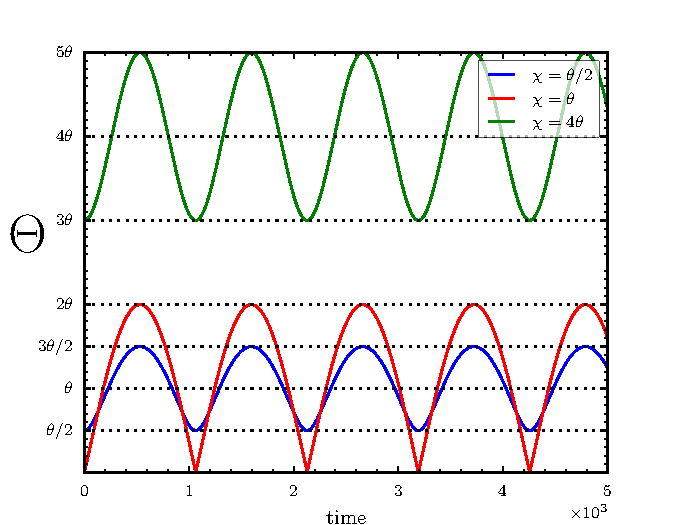
\includegraphics[width=0.7\textwidth]{polar_angle_variation_with_chi.pdf}
\caption{Variations in the polar angle of the dipole $\m$ under free precession}
\label{fig: polar angle variations}
\end{figure}

\section{Physical observables: pulse frequency}
The azimuthal angle $\Phi$ given in Eqn.~\eqref{eqn: Phi} gives us the phase of
the dipole. For the observer, the pulsation happens when the dipole passes through
the plane containing them and the angular momentum vector si we can always reorient
them such that the pulsation occurs every time $\Phi$ is a multiple of $2\pi$.
In this way, $\Phi$ is also the phase of the observed pulsations and as such
we can generate timing residuals from it; we will demonstrate this method in
Sec.~\ref{sec: timing residuals}.

The spin frequency of a pulsar is often used as a tool to study them, but when
precessing the observed frequency is not given by $\omega$ due to the
additional motions of precession. Instead, we note that the observer would
fit a timing model to the TOAs as the pulse passes through the plane containing
them and the angular momentum vector. So the frequency measured would be given
by the first derivative of $\Phi$:
\begin{equation}
\dot{\Phi} = \dot{\phi}
+ \frac{\sin\chi \left(
\dot{\psi} (\cos\theta\sin\chi - \sin \psi \sin \theta \cos\chi) +
\dot{\theta} \cos\psi (\cos\theta\cos\chi - \sin \psi \sin \theta \sin\chi)\right)
}{(\sin\theta \cos \chi - \cos \theta \sin \psi \sin \chi)^{2} + \cos^{2}\psi \sin^{2} \chi}.
\label{eqn: Phi_dot}
\end{equation}
This is the \emph{instantaneous electromagnetic frequency}, an observer
will measure the time averaged value of $\dot{\Phi}$ as the `spin frequency' of
the star.

In Fig.~\ref{fig: frequency variations} we plot the frequency modulations for the
three free precession cases considered in Fig.~\eqref{fig: polar angle variations}.
\begin{figure}[ht]
\centering
  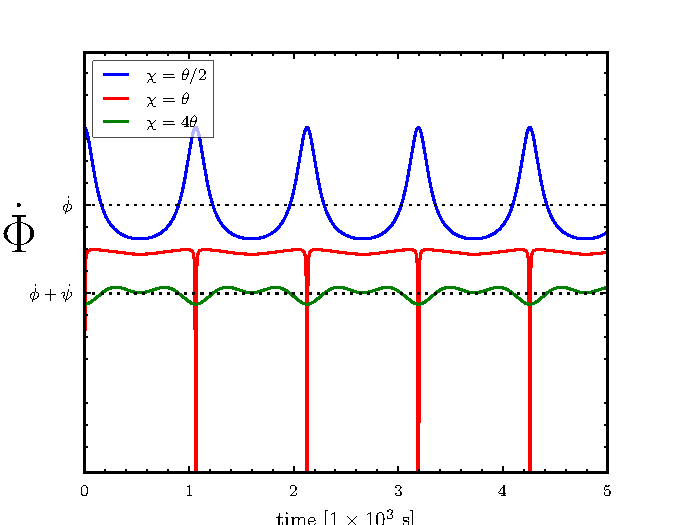
\includegraphics[width=0.7\textwidth]{frequency_variation_with_chi.pdf}
\caption{Variations in the spin-frequency of the dipole $\m$ under free precession}
\label{fig: frequency variations}
\end{figure}
Again this shows that free precession causes periodic modulations of the spin
frequency about an average value. To understand these and relate the spin
frequency to the underlying properties of the star, in the next section will
build an intuition for the motion of the dipole in the inertial frame.




%\subsection{Pulse frequency and polar angle under torqued precession}
%Having a physical understanding of why $\Theta$ and $\dot{\Phi}$ evolve under
%free precession as in Fig.~\ref{fig: polar angle variations} and Fig.~\ref{fig:
%frequency variations}, we will study what happens to such a system when
%including the effects of the EM torque.
%
%In Fig.~\ref{fig: polar angle variations with torque}  we give the variations in
%the polar angle under torqued precession.The torque introduces two
%additional effects: $\dot{\Phi}$ the instantaneous electromagnetic frequency
%decays slowly, this is caused by the spin down torque and is full agreement
%with what we expect; a fast sinusoidal oscillation in $\dot{\Phi}$ on the spin
%time scale, observable as a broadening of the line, is a result of the
%anomalous torque. As for the polar angle $\Theta$ the anomalous torque causes
%slight changes in the limits of the sinusoidal variation. Both the anomalous
%torque effects can be understood by realising that this effectively adds a
%triaxiality into the moment of inertia tensor. % needs more explanation
%
%\begin{figure}[ht]
%\centering
%	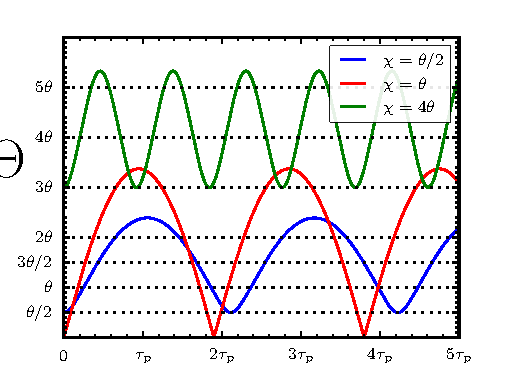
\includegraphics[width=0.7\textwidth]{polar_angle_variation_with_chi_inc_torque.pdf}
%\caption{Variations in the polar angle of the dipole $\m$ under torqued precession}
%\label{fig: polar angle variations with torque}
%\end{figure}
%
%\begin{figure}[ht]
%\centering
%	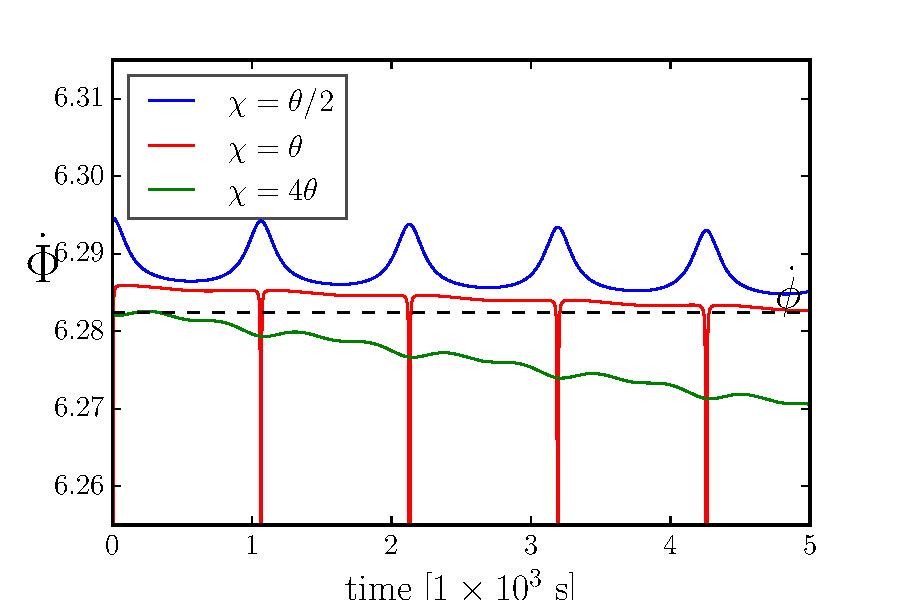
\includegraphics[width=0.7\textwidth]{frequency_variation_with_chi_inc_torque.pdf} \\
%\caption{Variations in the spin-frequency of the dipole $\m$ under torqued precession}
%\label{fig: frequency variations with torque}
%\end{figure}

\section{Physical observables: phase residuals}
\label{sec: timing residuals}

The principle observational quantify reported on for a pulsar is the timing
residual. This is measured by the difference between the TOA of a pulse and a
timing model of the pulsar as discussed in Sec.~\ref{sec: pulsar timing
methods}. It is the left over structure in the timing residual which we
term timing-noise and so in this section we will discuss how this can be calculated
from our numerical model. This will allow us to model timing residuals from
precessing pulsars, and add in new physics to understand how that effects the
timing residuals.

Using equation \eqref{eqn: Phi} we can calculate the exact phase evolution of
the star given the relevant Euler angles and components of the spin-vector; we
will label this as $\Phiexact$. Following the methods used by observers, we
then define our timing model as a
a Taylor expansion to the phase about some fixed time $t_{0}$
\begin{equation}
    \Phi(t; t_{0}, \phi, \f, \fdot, \fddot) =
    \phi + 2\pi \left(\f(t - t_{0}) +
                          \frac{\fdot}{2!}(t-t_{0})^{2} +
                          \frac{\fddot}{3!}(t-t_{0})^{3}
                          \right),
\label{eqn: TR taylor expansion}
\end{equation}
note that unlike observers we do not need to worry about other corrections such
as the motion of the Earth since $\Phiexact$ is given in the inertial frame.

We then use a least-squares fitting method to minimise the squared error
between the timing model Taylor expansion and $\Phiexact$. The resulting
coefficients $\{\phi_{0}, \f_{0}, \fdot_{0}, \fddot_{0}\}$ are the quantities
best describing the NS under a power law spin-down. We will refer to the
best-fit phase as described by  these coefficients as
\begin{equation}
    \Phifit(t) = \Phi(t; t_{0}, \phi_{0}, \f_{0}, \fdot_{0}, \fddot_{0})
\end{equation}
The phase-residual is then defined as the difference between the exact phase
and the fitted phase
\begin{equation}
  \Delta\Phi(t) = \Phiexact(t) - \Phifit(t).
\end{equation}
It is worth noting that a residual depends on which section of data was
used in the fit.

The phase residual can also be re-scaled to give the timing residual by
calculating the residual as a fraction of a cycle then multiplying by the
period
\begin{equation}
    \Delta T = \frac{\Delta\Phi(t)}{2\pi} P.
    \label{eqn: phase to timing}
\end{equation}
Over a typical observation periods it is possible for the period to
fractionally change due to the spin-down, but effect is negligible compared to
other variations. Therefore in this work we will report only on
phase-residuals.

\subsection{Effect of free precession on the phase residual}

\citet{Jones2001} analysed the geometric effect that precession will have on
the timing residual. This was done by considering the motion of the magnetic
dipole in the inertial frame as the superposition of motions due to the fast
rotation period and the slow precession. The results must be separated into the
two cases when $\theta > \chi$ and $\theta < \chi$. Of these two the authors
argue that `the wobble angle  of rapidly rotating stars are limited to small
values by the finite crustal breaking strain'. Therefore, the second case
$\theta < \chi$ holds greater physical relevance and so we focus on this region
of parameter space, although the simulation code is capable of finding solutions
for either. The phase residual for such NSs was shown to be given by
\begin{equation}
    \Delta\Phi^{49}(t) = -\wobbleangle \cot\chi\cos(\dot{\psi t}),
    \label{eqn: Jones 49}
\end{equation}
where the superscript here refers to the equation number from \citet{Jones2001}.
For a freely precession star $\dot{\psi}=\epsI \f$ is the constant free
precession frequency. Therefore, the magnitude of variations is given by
$|\Delta\Phi^{49}|=\wobbleangle \cot(\chi)$.

Equation \eqref{eqn: Jones 49} is calculated in the absence of any EM torque.
Nevertheless, it is still appropriate when such a torque is applied provided
that the geometric effect is stronger that any other (these are discussed in
the next few sections). As such we begin by simulating a NS with the properties
listed in table \ref{tab: PR 49}. Nonphysical values of the
rotation frequency and magnetic field have been used to aid the computational
speed. The resulting phase residual, in cycles, is given in figure \ref{fig:
PR 49}.

\FigureAndTable{49_verification}{PR 49}{
The phase residual in cycles for a simulated NS with the properties described
in the table. This is used to illustrate the
agreement with the magnitude of variations from equation \eqref{eqn: Jones 49}
taken from \citet{Jones2001}.}


\subsection{Effect of torqued precession on the phase residual}
\label{sec: phase residual torqued}
Considering a vacuum point-dipole spin-down torque \citet{Jones2001} found that
the EM torque can amplify the geometric effect of equation \eqref{eqn: Jones
49}. The magnitude of variation due to EM torque is given by
\begin{equation}
    |\Delta\Phi^{63}| = \frac{1}{\pi}\left(\frac{\tau_{P}}{P}\right)
    \left(\frac{\tau_{P}}{\tau_{S}}\right)
                                    |\Delta\Phi^{49}|
\label{eqn: Jones 63}
\end{equation}
The two ratios of time-scales define an `amplification factor':
\begin{equation}
    \mathcal{A}_{\mathrm{EM}} = \left(\frac{\tau_{P}}{P}\right)
                                \left(\frac{\tau_{P}}{\tau_{S}}\right)
\label{eqn: EM amplification}
\end{equation}
The amplification increases
the magnitude of phase residuals for young pulsars with short periods.

We simulate such a star using the properties in table \ref{tab: 63} noting that
the amplification factor is $\sim 3$ when including the factor of $\pi$. The
resulting phase residual is plotted in figure \ref{fig: PR 63} along with the
magnitude of variations due to free precession along and the amplification due
to the EM torque. The magnitude of the simulated phase-residuals are found to
agree well with the analytic results of equation \eqref{eqn: Jones 63}.

\FigureAndTable{63_verification}{PR 63}{
The phase residual in cycles for a simulated NS with the properties described
in table \ref{tab: 63 verification properties}. This is used to illustrate the
agreement with the magnitude of variations from equation \eqref{eqn: Jones 63}
taken from \citet{Jones2001}.}

%In figure \ref{fig: TR no torque} we plot the timing residuals as calculated in
%the torque free model for three values of $\chi$. It is worth noting that the
%power law spin down assumes that the star is in fact spinning down; without the
%torque this model can't not spin down. We can however interpret these results
%as the effect of precession on timing residuals in the limit for which the
%variation due to precession is much stronger than the spin down.
%%\begin{figure}[ht]
%%\centering
%%	\includegraphics[width=0.7\textwidth]{Timing_residuals_no_torque.pdf}
%%\caption{Plot of the timing residuals for three angles of $\chi$ in the torque
%%         free model showing different types of behaviour. }
%%\label{fig: TR no torque}
%%\end{figure}
%The results show that the precession induces a periodic variation on the
%precession timescale, the magnitude is proportional to the angle $\chi$. We
%also find the results are dependant on the initial angle $a_{0}$.

\subsection{Effect of torqued precession on the phase residual: orthogonal rotator}

In analysing observations of free precession \citet{Jones2001} applied the
model to PSR B1821-11: a pulsar with a strongly periodic residual that has been
cited as a strong candidate for free precession \citet{Stairs2000}. From the
variations in pulse shape an estimate can be made of the wobble angle
$\wobbleangle \sim 3^{\circ}$. Finding that the amplification factor was
important for this pulsar (it can be calculated to be $\approx 380$),
\citet{Jones2001} attempted to extract the wobble
angle by inverting \eqref{eqn: Jones 63}. This yields a wobble angle that
disagreed with the estimation from a pulse shape variations. The author
concluded that the strong harmonic periodicity's suggested the dipole was
nearly orthogonal e.g. $\chi \approx \pi/2$.  This required expansions of the
phase modulation resulting in an estimate
\begin{equation}
    |\Delta\Phi^{75}| = \frac{1}{4\pi} \frac{\tau_{P}^{2}}{\tau_{S} P} \theta^{2}
    \label{eqn: Jones 75}
\end{equation}

In figure \ref{fig: PR 75} we simulate the B1828-11 pulsar taking the values
from \citet{Stairs2000} and modifying them to allow the simulation to complete
in a reasonable time. The modification was setup such that the amplification
factor remained the same along with the ratio of timescales. The properties
of the simulation are given in \ref{tab: 75}

\FigureAndTable{75_verification}{PR 75}{
The phase residual in cycles for a simulated NS with the properties described
in table \ref{tab: 75 verification properties}. This is used to illustrate the
agreement with the magnitude of variations from equation \eqref{eqn: Jones 75}
taken from \citet{Jones2001}.}

\section{Physical observables: spin-down rate $\dot{\nu}$}
An observable which is often considered in characterising periodic patterns in
pulsar signals is the spin-down rate $\spindown$. In our numerical model, the
spin-down rate is the same as the second derivative of the magnetic dipoles
azimuthal angle (i.e. $\ddot{\Phi}$).

As we will now show, the spin-down rate is modulated by free precession, but
this effect can also be amplified by the electromagnetic torque in the same way
the timing residuals modulations were amplified in the previous section.
In order to understand all of the subtle physics which
may be present in the spin-down rate, we will now build our intuition by starting
with the simplest models and gradually introducing new features.

Calculation of the spin-down rate can be done in two ways: either analytically
building on results from \citet{Jones2001}, or we can numerically solve the
system of equations and measure the spin-down rate (discussed shortly). Using the
latter method we include by default all of the interplay between precession and
the EM torque. We then compare this `exact' solution with analytic results
which allows us to understand which parts of the system are responsible for the
observed phenomena.

In order to calculate the spin-down rate from numerical solutions we could
numerically differentiate eqn.~\eqref{eqn: Phi} (the angular phase of the
magnetic dipole). However, since we are comparing our results with measured
values from pulsar astronomers, an alternative is use the method proposed by
\citet{Lyne2010}: a second order Taylor expansions is fitted to short sections
of data of length $T$ and the resulting coefficient $\spindown$ is recorded the
mid-point in time of the section of data. Repeating this process every $\sim
T/4$ in a `sliding-window', we build a picture of how the spin-down varies with time.
In the following our numerical results will use this technique which we refer
to as the \emph{Lyne-method}.
We choose $T$ such that it is a fraction of the precession period over which we
expect quantities to be modulated. This is consistent with the observers method
where $T$ is chosen in order to resolve the observed modulations.

We now proceed to compare this numerical spin-down rate calculation with analytic
predictions gradually introducing new features when required. Since the geometric
variations can be quite complex, we consider only $\theta < \chi$ and start
with $\theta \approx 3^{\circ}$ and $\chi=60^{\circ}$. This produces simple
simple oscillatory behaviour. The solution become more complex if either
the inequality is not satisfied or $\chi \approx \pi/2$ which we will not
consider here.

\subsection{Spin-down variations due to free-precession}
\label{sec: spin-down free precession}

Without an EM torque, the average spin-down rate should be zero. However, if
the body undergoes free precession, this will produce periodic variations.
These can be calculated exactly by differentiating Eqn. \eqref{eqn: Phi_dot}
twice. Since the system is torque free, we have $\dot{\theta} = 0$ leaving
\begin{equation}
    \ddot{\Phi}(t)_{\mathrm{p}} = \ddot{\phi} + \frac{d}{dt}\left(
        \sin\chi\dot{\psi} \frac{\cos\theta\sin\chi - \sin \psi \sin \theta \cos\chi
}{(\sin\theta \cos \chi - \cos \theta \sin \psi \sin \chi)^{2} + \cos^{2}\psi \sin^{2} \chi}
\right)
\label{eqn: Phi_ddot FP}
\end{equation}
The expanded expression is unwieldy and so we do not report it here. For a
freely precessing biaxial body we demonstrated in Sec.~\ref{sec: biaxial body
with no torque} that, in the absence of any torque, the Euler angles evolution's
are linear functions of time. As such the first term in this expression
vanishes and we are left with a complicated trigonometric function of $\psi(t)$
which is given by Eqn.~\eqref{eqn: euler angles torque free evolution}.

It is also useful to calculate the magnitude of variations: this is done by
differentiating Eqn.~\eqref{eqn: Jones 49} twice giving
\begin{equation}
    |\Delta\spindown|_{\mathrm{p}} =\frac{\dot{\psi}^{2} \theta \cot\chi}{2\pi}.
    \label{eqn: spin-down variations FP}
\end{equation}

In Fig.~\ref{fig: nu_dot no torque} we plot three curves: the numerical
result obtained using Lyne-method of calculating the spin-down, the analytic
prediction from Eqn.~\eqref{eqn: Phi_ddot FP}, and the magnitude obtained by
Eqn.~\eqref{eqn: spin-down variations FP}.
\FigureAndTable{nu_dot_no_torque}{nu_dot no torque}{ Modulations in the
    spin-down rate due to free precession. The solid black line is the numerical
    solution, in blue we show the analytic prediction of the magnitude of
    modulations due to free-precession as given by Eqn.~\eqref{eqn:
    spin-down variations FP}, and the red-dashed line indicates the analytic
    prediction of Eqn.~\eqref{eqn: Phi_ddot FP}}
The variations seen in Fig.~\ref{fig: nu_dot no torque} are the result of
free precession. As there is no torque, the average spin-down rate is zero. However,
due to precession the magnetic dipole performs a slow rotation about the
deformation axis. During half the cycle it counter-rotates and in the other
half it corotates with the rapid rotation about the angular momentum vector.
The result is a symmetric modulation of the spin-down rate about zero with magnitude
given by Eqn.~\eqref{eqn: spin-down variations FP}.

\subsection{Spin-down variations due to torqued precession}
In this section we will develop analytic models for the periodic variations
due to precession under an EM torque. This problem has been considered before
in the context of PSR~B1828-11 \citep{Jones2001, Link2001, Akgun2006}, we will
expand on these results and compare the analytic models with the numeric
results calculated using the Lyne-method.

\subsubsection{Average spin-down rate}
When we include the EM torque we will have a non-zero average spin-down rate.
We can calculate this directly from Eqn.~\eqref{eqn: surface magnetic field}:
rearranging for $\dot{\Omega}$ we have
\begin{equation}
    \dot{\Omega} = -\frac{B_{0}^{2}R^{6} \sin^{2}\alpha \Omega^{3}}{6I_{0}c^{3}},
\end{equation}
written in terms of the model parameters this is
\begin{equation}
\dot{\nu} = -\frac{1}{3\pi}\frac{R \Omega^{3}}{c} \sin^{2}\alpha \epsA.
\end{equation}

In the dipole spin-down model the second-order spin-down rate is given
approximately by
\begin{align}
\ddot{\nu} \sim \frac{|\dot{\nu}|}{\tauAge}
\end{align}
As the spin-down age of typical neutron stars is much longer that
the time which we observe pulsars for $\sim 10$~yrs, the variations in $\dot{\nu}$
due to $\ddot{nu}$ are typically small. Therefore, we can take the initial value
of $\dot{\nu}$ as a good estimate for the average spin-down rate
\begin{align}
\langle\dot{\nu}\rangle \approx -\frac{1}{3\pi}\frac{R \Omega_{0}^{3}}{c} \sin^{2}\alpha \epsA
    \label{eqn: spin-down initial EM}
\end{align}
In this expression, $\alpha$ is the angle between the spin-vector and the
magnetic dipole. For small wobble angles, the angle $\hat{\theta}$ (see figure
\ref{fig: reference plane}) is vanishingly small and so we can approximate
$\alpha \approx \chi$ such that the average spin-down rate is
\begin{equation}
    \langle \dot{\nu}\rangle = -\frac{1}{3\pi}\frac{R \Omega_{0}^{3}}{c} \sin^{2}\chi \epsA
    \label{eqn: spin-down average}
\end{equation}

This expression will give us the average spin-down under an EM torque; if the
star precesses, then the actual spin-down will be modulated about this values
due to precession. Before demonstrating how to calculate this modulation we
first show that the magnitude of modulation will depend on the EM torque.

\subsubsection{Amplification of the spin-down modulation}

For the timing residuals \citet{Jones2001} demonstrated that the residuals
could be amplified by the EM torque by the factor given in Eqn.~\ref{eqn: EM
amplification}. We now show that the same effect applies
to the spin-down modulation.


Starting with a vacuum point-dipole spin-down torque \citet{Jones2001}
demonstrated that the magnitude of modulations of the spin-down rate under is
\begin{equation}
    |\Delta\ddot{\Phi}|^{58} \approx -2k\Omega^{3} \theta \sin\chi \cos\chi,
\end{equation}
here the superscript refers to the relevant equation in \citet{Jones2001}. Taking
this expression, we now show that it can be rewritten
\begin{align}
    |\Delta\ddot{\Phi}|^{58}
    & \approx 2k\Omega^{3} \theta \sin\chi \cos\chi & \\
    & \approx 2 \frac{\ddot{\Phi}}{\sin^{2}\alpha} \theta \sin\chi\cos\chi &
    \mathrm{if }\; \alpha \approx \chi \\
    & \approx 2 \ddot{\Phi}\theta \cot\chi &
    \tauS = \left| \dot{\Phi} / \ddot{\Phi}\right| \\
    & \approx 2 \frac{\dot{\Phi}}{\tauS} \theta \cot\chi &
    P/\tauP = \dot{\psi}/\dot{\Phi} \\
    & \approx 2 \dot{\psi}^{2}\left(\frac{\tauP}{P}\right) \frac{1}{\dot{\psi}} \frac{1}{\tauS} \theta \cot \chi & \dot{\psi} = \frac{2\pi}{\tauP} \\
    & \approx \frac{1}{\pi}\dot{\psi}^{2}\left(\frac{\tauP}{P}\right)\left(\frac{\tauP}{\tauS}\right) \theta \cot\chi
    \label{eqn: spin-down variations FP EM}
\end{align}
Here we have shown that, just like for the timing residuals, the EM torque can
amplify the spin-down modulation by a factor $\mathcal{A}_{\mathrm{EM}}$ as
defined in Eqn.~\eqref{eqn: EM amplification}. In the following two sections
we will investigate how precession effects the spin-down rate with and without
this amplification factor.

\subsubsection{Geometric dominated spin-down modulation}

When $\mathcal{A}_{\mathrm{EM}} \ll 1$, the geometric variations in the
spin-down studied in Sec.~\ref{sec: spin-down free precession} will dominate.
We can derive an ad-hoc analytic expression by allowing
$\ddot{\phi}$ in Eqn.~\eqref{eqn: Phi_ddot FP} to be non-zero and given
exactly by $\ddot{\phi} = 2\pi\langle\dot{\nu}\rangle$, where the average
rate is given in Eqn.~\eqref{eqn: spin-down average}. Combining this with the
geometric modulations, the analytic prediction is given by
\begin{equation}
    \ddot{\Phi}(t) = 2\pi \langle\dot{\nu}\rangle + \frac{d}{dt}\left(
        \sin\chi\dot{\psi} \frac{\cos\theta\sin\chi - \sin \psi \sin \theta \cos\chi
}{(\sin\theta \cos \chi - \cos \theta \sin \psi \sin \chi)^{2} + \cos^{2}\psi \sin^{2} \chi}
\right)
\label{eqn: 1238}
\end{equation}
We verify this analytic expression in Fig.~\ref{fig: nu_dot with torque} where
we plot a typical spin-down calculation with $\mathcal{A}_{\mathrm{EM}} \approx
0.4$. Here we see  the non-zero average spin-down (given by Eqn.~\eqref{eqn:
spin-down average}) due to EM torque modulated by the geometric variations of
free precession. The black (numerical results) and dashed red lines (analytic
prediction) show good agreement.

\FigureAndTable{nu_dot_with_torque}{nu_dot with torque}{
Modulation in the spin-down rate due to precession. The solid black line
indicates the numerical solution including a torque; the solid red line indicates
the approximate average spin-down rate due to the EM toque as calculated
from equation \eqref{eqn: spin-down initial EM chi}; the blue lines indicate
the magnitude of modulation about the average spin-down due to precession; finally
the red-dashed line is the prediction of Eqn.~\eqref{eqn: 1238}.}.

\subsubsection{EM torque amplification of the spin-down modulation}
When $\Aem$ is greater than unity the spin-down modulations are amplified by
the torque. We can generate an analytic prediction for this by substituting
Eqn.~\eqref{eqn: Phi_dot} and Eqn.~\eqref{eqn: Theta 2} into the vacuum point-dipole spin-down
torque:
\begin{align*}
\ddot{\Phi} = {} & k \dot{\Phi}\sin^{2}\Theta \\
            = {} & -\frac{2R}{3c} \epsA
                   \left(\dot{\phi}
                         +\frac{\dot{\psi}\sin(\chi)
                                (\cos\theta\sin\chi - \sin \psi \sin \theta \cos\chi)
                               }{
                                (\sin\theta \cos \chi - \cos \theta \sin \psi \sin \chi)^{2}
                         + \cos^{2}\psi \sin^{2} \chi}\right)^{3} \\
            &  \hspace{18mm}  \times  \sin^{2}\left(\cos^{-1}\left(
                     \sin\theta\sin\psi\sin\chi + \cos\theta\cos\chi\right)\right)\\
    = {} & -\frac{2R}{3c} \epsA
    \left(\dot{\phi}+\frac{\dot{\psi} \sin(\chi)(\cos\theta\sin\chi
          -\sin \psi \sin \theta \cos\chi)}
         {(\sin\theta \cos \chi - \cos \theta \sin \psi \sin \chi)^{2}
         + \cos^{2}\psi \sin^{2} \chi}\right)^{3} \\
   & \hspace{18mm} \times \left(\sin\theta\sin\psi\sin\chi + \cos\theta\cos\chi\right)
\end{align*}
where we are implicitly assuming $\theta=\mathrm{const.}$, this is not true
when we include the EM torque. However, provided the variations are small we
can assume it as a first approximation.  Finally, we assume that the Euler angles
are approximately the same as in the torque free case, that is:
\begin{align}
    \phi(t) = \omega_{0}t + \phi_{0} &&& \psi(t) = -\epsI \omega_{0} t + \pi/2
\end{align}

 \begin{align}
\begin{split}
     \ddot{\Phi} =&-\frac{2R}{3c} \omega_{0}^{3}\epsA
     \left(1 -  \epsI\frac{ \sin(\chi)(\cos\theta\sin\chi - \sin \psi \sin \theta \cos\chi)
     }{(\sin\theta \cos \chi - \cos \theta \sin \psi \sin \chi)^{2} + \cos^{2}\psi \sin^{2} \chi}\right)^{3}\\
     &\hspace{22mm}\times\left(\sin\theta\sin\psi\sin\chi + \cos\theta\cos\chi\right)
     \label{eqn: Phi_dot EM}
\end{split}
\end{align}
In Fig.~\ref{fig: nu_dot with torque EM} we plot the results of a simulation
for which this amplification factor is greater than unity. This confirms that the
spin-down variations are given by Eqn.~\ref{eqn: spin-down variations FP EM} rather
than Eqn.~\eqref{eqn: spin-down variations FP}.

\FigureAndTable{nu_dot_with_torque_EM_amplification}{nu_dot with torque EM}{
EM amplification of the modulation in the spin-down rate due to precession.
The solid black line indicates the numerical solution including a torque; the
solid red line indicates the approximate average spin-down rate due to the EM
toque as calculated from equation \eqref{eqn: spin-down average}; the
blue region indicates the modulation about the average spin-down due to
precession from Eqn.~\eqref{eqn: spin-down variations FP} while the green
region indicates the modulation about as calculated from
Eqn.~\eqref{eqn: spin-down variations FP EM}.}


\section{Physical observables: pulse intensity}
\label{sec: intensity}
Assuming a fixed magnitude of the magnetic dipole, the pulse amplitude will
depend on the orientation of the magnetic dipole to the observer and the
beam geometry. It will be
maximal when pointing directly at the observer and presumably fall off as the
angle between the two grows. To model this we take an observers position as
$\Phi_{O}, \Theta_{O}$ and then assume the beam geometry follows
Gaussian profile with a single conal emission. This could later be adapted
to include a coral emission.

For such a model of the the beam geometry, the pulse amplitude will vary with the
angular separation of the vector from the centre of the star to the observer and the
magnetic dipole vector. BY considering the intersection of these vectors with
the unit sphere, the angular separation can be shown to be
\newcommand{\ThetaO}{\Theta_{\mathrm{obs}}}
\newcommand{\PhiO}{\Phi_{\mathrm{obs}}}
\newcommand{\sigmaB}{\sigma_{B}}
\begin{equation}
\Delta\sigma = \cos^{-1}\left(\sin(\Theta)\sin(\ThetaO) +
                             \cos(\Theta)\cos(\ThetaO)\cos(\Phi - \PhiO)\right)
\label{eqn: angular sep inv cos}
\end{equation}
Then the amplitude of the pulse will be given by
\begin{equation}
A(\Theta, \Phi, \ThetaO, \PhiO, \sigmaB) =
A_{0} \exp\left(-\frac{\Delta\sigma^{2}(\Theta, \Phi, \ThetaO, \PhiO)}{2\sigmaB^{2}}\right)
\label{eqn: beam amplitude}
\end{equation}
where $A_{0}$ is some constant amplitude, $\sigmaB$ is a measure of the
angular beam width.

In figure \ref{fig: amplitude variation} an illustration is given of variations
in amplitude from a torque-free pulsar with some arbitrary parameters. This is
intended to demonstrate the fast rotation frequency of individual pulses, along
with the longer modulation of the precession.
\begin{figure}[htb]
\centering
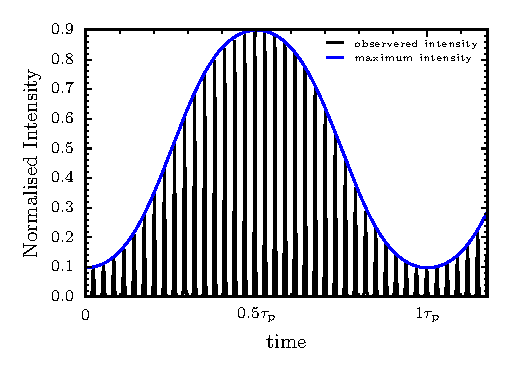
\includegraphics[width=.7\textwidth]{intensity_variation}
\caption{Amplitude variation using a 2D Gaussian emission.}
\label{fig: amplitude variation}
\end{figure}•

%\begin{equation}
%A(\Phi, \Theta) = A_{0} \textrm{exp} \left(
%                         -\frac{\tilde{\Phi}^{2}}{2\sigma_{\Phi}^{2}}
%                         -\frac{\tilde{\Theta}^{2}}{2\sigma_{\Theta}^{2}}
%                                     \right)
%\label{eqn: Amplitude}
%\end{equation}•
%where $\tilde{\Phi}=\mod_{2\pi}(\Phi)-\Phi_{O}$ and
%$\tilde{\Theta}=\mod_{\pi}(\Theta) - \Theta_{O}$. Computing the angles $\Phi$ and $\Theta$ from numerical
%solutions of the original ODEs and using the above emission model gives
%the pulse amplitude as seen be an observer. An example of a solution showing
%the individual pulses along with the modulation due to free precession is
%given in figure \ref{fig: amplitude_variation}

\section{Application: switching and precession}

Recently, some workers in the field \citep{Lyne2010, Perera2015} are suggesting
that quasi-periodic structure observed in pulsar timing residuals is a result
of magnetospheric torque-switching events as described in Sec.~\ref{sec: two
state switching}. In such models, the spin-down periodically switches between
two distinct values and these changes correlate with changes in the beam-width.
These models however are lacking a key feature: the clock which provides the
periodicity. It has been suggested \citep{Jones2012} that it may in fact be
precession which provides this clock. Ultimately, the numerical model developed
in this section could study this effect. For example by implementing a hybrid
model in which propensity for a magnetospheric switch to occur is related to
the angle $\Theta$. In this way, the observed switching would undergo
stochastic resonance as suggested by \citet{Cordes2013} (see Appendix~\ref{App
Stochastic} for further details).

In this section we will present preliminary results on a simplified hybrid model
in which we consider single switching events. We will not connect the switching
to precession, but simply consider a single switch in the torque at some time
$t_{\mathrm{switch}}$; for the time being we set this to be half the
observation period, such that $t_{\mathrm{switch}} = \To/2$.

In the EM dipole spin-down model the torque has two distinct components: the
regular spin-down part and the so-called anomalous component. This later term 
does not contribute to the spin-down, but as discussed in section \ref{sec: effective
body frame} it will modify the axis of precession. The torque switching will 
occur in the spin-down component, but it seems unlikely that it will also
occur in the anomalous component [Ian - why?]. To cover all cases we 
model a single torque switching effect by redefining the torque in equation
\eqref{eqn: torque} such that

\newcommand{\Ss}{S_{\mathrm{S}}}
\newcommand{\Sa}{S_{\mathrm{A}}}

\begin{equation}
\mathbf{T} = (1 - \Ss H(t-t_{\mathrm{switch}})) \mathbf{T}_{\mathrm{S}}+
                 (1 - \Sa H(t-t_{\mathrm{switch}})) \mathbf{T}_{\mathrm{A}}
\label{eqn: single switch torque}
\end{equation} 
where the subscripts label the spin-down and anomalous components, $S$ is the
strength of switching, and $H(t)$ is the Heaviside function. 

Numerically solving the body-frame and Euler equations using this torque we 
simulate a single switching event to try and understand the effect it will have
on phase residuals. 

\subsubsection{Minimal precession}
Without the torque-switching, in these simulations only free precession can 
produce structure in the phase residuals. No pulsars exist with regular periodic
structure that can be solely interpreted as free precession. Most pulsars must 
therefore exist with very small wobble angles with any excitement of this being
damped. As such, we begin by discussing the "minimal precession" initial 
conditions from which to start our simulations. 


Precession will not occur when the spin vector is aligned with the axis about
which it rotates. The angle between these two we have defined as the wobble
angle.  For minimal precession we should therefore set this wobble angle to
zero. In all simulations we consider a biaxial body with the full torque given
in \eqref{eqn: single switch torque}. From our previous discussion on the 
wobble angle we can minimise the precession by setting the initial polar angle
of the spin vector in the body frame to lie along the effective body-frame 
axis. That is
\begin{equation}
a_{0} = \beta(\epsI, \epsA, \chi),
\end{equation}
we refer to such a simulation as `minimal precession' since the wobble angle 
remains non-zero.

In this case the wobble angle will given by equation \eqref{eqn: spin-down wobble angle}:
The magnitude of variations in the phase-residuals is given by inserting this
wobble angle
\begin{equation}
\wobbleangle \approx \frac{1}{\epsI}{\frac{P}{\tauS}}
\end{equation} 
into either equation \eqref{eqn: Jones 49} or \eqref{eqn: Jones 75} depending 
on the EM amplification factor.

We verify this by setting up a minimal precession simulation. The resulting
phase residual is given in figure \ref{fig: no switching} along with the
predicted magnitude of variations. In table \ref{tab: NoSwitching properties}
we give the simulation properties: note that the initial polar angle is exactly
the angle $\beta$ which can be calculated using equation \eqref{eqn: beta}. 
The wobble angle is given by equation \eqref{eqn: wobble angle} and is non-zero
due to the spin-down torque. 

\begin{figure}[htb]
\begin{floatrow}
\ffigbox{%
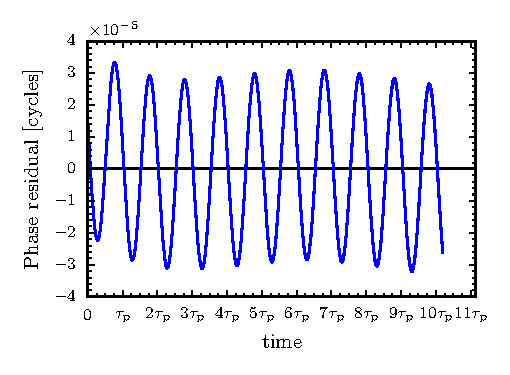
\includegraphics[width=0.5\textwidth]{NoSwitching.pdf}
}{%
    \caption{}
  \label{fig: no switching}
}
\capbtabbox{%
  \begin{tabular}{ccl}
\multicolumn{3}{c}{Simulation parameters} \\
\hline
$\omega_0$  &=& 100 rad/s\\
$B_0$  &=& $10^{15}$ G \\
$\chi$  &=& 50$^{\circ}$ \\
$a_0$ &=& -0.78$^{\circ}$ \\
$\mathcal{A}_{\mathrm{EM}}$ &= & $23$
\end{tabular}

}{%
  \caption{}%
  \label{tab: NoSwitching properties}
}
\end{floatrow}
\end{figure}


We will now setup a simulation of this `minimal precession` NS, and then 
manually switch the torque. We choose a NS where the EM torque amplification
given in equation \eqref{eqn: Jones 75} is important.

\subsection{Switching without the anomalous torque}
We now consider manually switching the spin-down torque halfway though the simulation.
That is we set
\begin{align}
    t_{\mathrm{switch}} = \frac{\To}{2}, &&& \Ss = 0.4, &&& \Sa = 0.0,
\end{align}
such that halfway though the simulation the spin-down torque is reduced by a
fraction $0.4$ while the anomalous torque remains unaffected. 

In figure \ref{fig: switching without anom} we plot the phase residuals from
this simulation. In the top plot is the residual as calculated over the entire
observation period. We find a single periodic variation with significantly
larger variation than any of the precession features. This is a direct result
of the switching only% as discussed in section \ref{sec: Lyne two state}:
the
effect of precession is entirely swamped by the switching. For this reason in
the lower plot we calculate two residuals: the first is calculated
in the region $[0, t_{\mathrm{switch}}]$ and the second in $[t_{\mathrm{switch}}, \To]$.
Because the switch does not occur in either of these periods we can resolve the
free precession during each period.

\begin{figure}[htb]
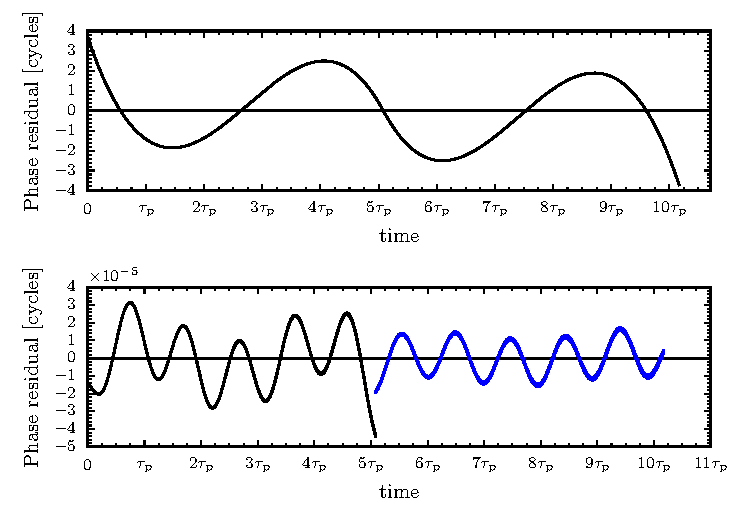
\includegraphics[width=.5\textwidth]{SwitchingWithoutAnomTorque}
\caption{}
\label{fig: switching without anom}
\end{figure}

The simulations begin in the minimal precession state where the spin-vector
is aligned with the effective body frame axis such that the wobble angle is given
by equation \eqref{eqn: spin-down wobble angle}. After the switch, the wobble
angle is smaller by a factor $\Ss$ and as a result we see the precession is
reduced by this fraction.


\subsection{Switching with the anomalous torque}
We now consider manually switching both the spin-down and anomalous torque
halfway though the simulation.  That is we set
\begin{align}
    t_{\mathrm{switch}} = \frac{\To}{2}, &&& \Ss = \Sa = 0.01
\end{align}

In a similar fashion to figure \ref{fig: switching without anom} we show first
the total residual in the top plot of figure \ref{fig: switching with anom}, and
then the individual residuals in the lower plot.

In this simulation we have used a significantly smaller switching fraction 
than when switching without the anomalous torque. This is because the effect 
on the phase residuals when calculated in the two regions is significantly
stronger. This is because we begin with a `minimal precession' state, where
$\theta = \beta$ and the precession results from effect of the spin-down torque.
Then, when we switching off a fraction of the anomalous torque we have modified
the effective body frame and hence the angle $\beta$. This generates a significantly
larger wobble angle producing a significant increase in the phase residuals
fitted in the post-switch period. The effect is not observable when fitting
to the entire simulation period since the switching event remains dominant.

\begin{figure}[htb]
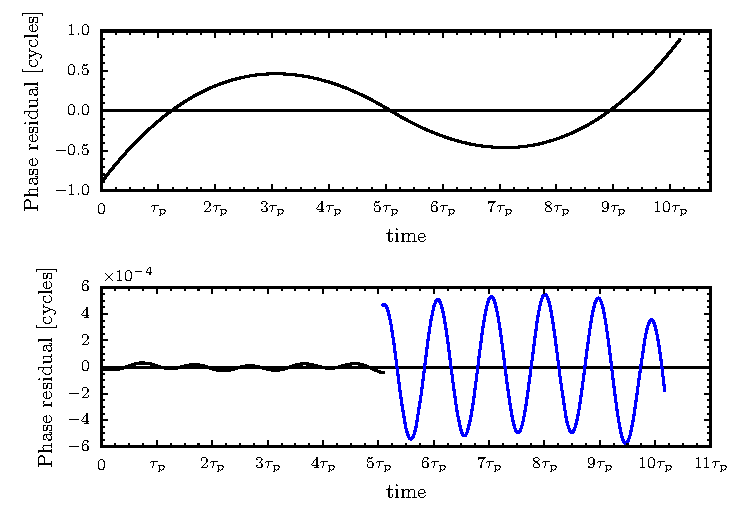
\includegraphics[width=.5\textwidth]{SwitchingWithAnomTorque}
\caption{}
\label{fig: switching with anom}
\end{figure}

\subsubsection{Calculating the new wobble angle after a switch}
We now calculate the change in wobble angle and hence phase-residual variations
after switching a fraction of the anomalous torque.
In our model the strength of the torque is parameterised
by $\epsA$, related to the surface magnetic field strength by 
\begin{align}
    \epsA = \frac{R^{5}}{4I_{0} c^{2}} B_{0}^{2}.
\end{align}
Rearranging equation (1.4.8) of my transfer thesis we can then write the 
spin-down as 
\begin{align}
    \dot{\omega}_{0} & = -\frac{B_{0}^{2}R^{6} \sin^{2}(\alpha) \omega_{0}^{3}}{6 I_{0} c^{3}} \\
    & = - \frac{2 R \epsA \sin^{2}(\alpha) \omega_{0}^{3}}{3 c},
\end{align}
where $\alpha$ is the angle between the spin-vector and magnetic dipole. Since
we expect these to be misaligned in order to observe pulsations, we can take
$\sin^{2}\alpha \approx 1$.
Taking the spin frequency as a fixed value yields an estimate for the
spin-down frequency
\begin{equation}
    \fdot = - \frac{R\omega_{0}^{3}}{3\pi c}\epsA.
    \label{eqn: spin-down of epsA}
\end{equation}

In the two-state switching model, the spin-down value was observed to change
by a fraction $\upsilon$ such that
\begin{equation}
    \fdot \rightarrow \fdot' = (1-\upsilon)\fdot,
\end{equation}
then from equation \eqref{eqn: spin-down of epsA} 
\begin{equation}
    \epsA \rightarrow \epsA' = (1-\upsilon)\epsA.
\end{equation}

The two-state switching changes the value of $\epsA$ and so has a knock-on 
effect on the effective body frame. A non-precessing NS at an
angle $\beta(\epsI, \epsA, \chi)$ will, after a torque switch by a fractional
amount $\upsilon$, no longer be aligned with the body frame axis. This is 
because the effective body frame will have shifted to 
$\beta' = \beta(\epsI, \upsilon\epsA, \chi)$. As a result, we should expect the
previously non-precessing NS to begin precessing after a torque switching event. 

The NS will precess at the usual precession frequency in a cone  of half-angle
\begin{equation}
    \Delta\beta(\epsI, \epsA, \chi, \upsilon)=|\beta - \beta'|,
\end{equation}
about the new effective body-frame axis.  The expression for $\Delta \beta$ is
not easily amenable to manipulation, but can easily be explored graphically.
This is done in figure \ref{fig: DeltaBetaPlot} for several choices of
$\upsilon$. This illustrates that the precession angle can be as much as a few
degrees although it tends to zero in the limit $\epsI \gg \epsA$.

\begin{figure}[htb]
    \centering
    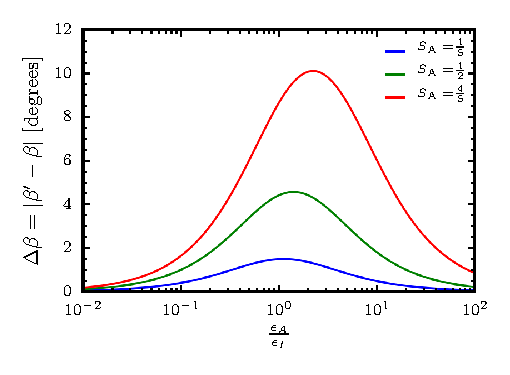
\includegraphics[width=0.5\textwidth]{DeltaBetaPlot}
    \caption{Illustrating the magnitude of the precession angle after switching
        due to the new rotation of the effect body frame. We plot the half-angle
        ($\Delta\beta$) of the precession cone as a function of the ratio
    $\epsA/\epsI$. Typically we expect real stars to have $\epsA < \epsI$.}
    \label{fig: DeltaBetaPlot}
\end{figure}

Since it is hard to gauge the significance of this we will apply it to the
PSR B1828-11; a pulsar which demonstrated evidence for precession \citet{Stairs2000}
and has since been reinterpreted as two-state switching \citep{Lyne2010}. This
has a frequency of $\f = 2.47$~Hz, a spin-down $\fdot=-3.65\times10^{-13}$~Hz/s, switches are
observed to occur every $T\approx 1.4$ yrs, and the spin-down changes by $\upsilon = 0.71$.

We are unable to directly calculate $\Delta\beta$ from this information, since
we do now know $\epsI$ or $\chi$. Nevertheless, we can at least find the maximum
allowed value found when $\chi \ll 1$ and $\epsI \sim \epsA$. This has not 
been found exactly although it could easily be done by maximising the function 
numerically. Approximately the maximum allowed angle is $\Delta\beta \sim 45^{\circ}$.

We can now attempt to quantify the effect this may have on the timing residuals.
Precession, as shown by \citet{Jones2001}, will produce a sinusoidal variation
in the residual with a magnitude given by 
\begin{equation}
    \Delta\Phi_{\mathrm{FP}} \sim \pi \cot(\chi) \theta.
\end{equation}
This precession will be damped by other processes, but in the immediate aftermath
of a switch, may be detectable. 

However, when considering the residual which includes a switch we must also
take into account the effect this will have. This was considered in section (6.6)
of my transfer thesis. Here we present the result that, the maximal size of phase-residuals
assuming several switched occur during an observation is given by 
\begin{equation}
    \Delta\Phi_{\mathrm{TS}} \sim \frac{\pi}{16} \upsilon \fdot  T^{2},
\end{equation}
Where $T$ is the switching period

For PSR B1828-11 then we can directly compute the magnitude of variations in
the timing residual:
\begin{align}
    \Delta t_{\mathrm{TS}}^{\mathrm{B1828-11}} \approx 70\mathrm{~ms}
\end{align}
This is considerably larger than the result from \citet{Lyne2010} who measured a 
peak to peak residual of 94 ms.


\biblio

\end{document}
